\chapter{Introduction}
\label{ch:introduction}

Progress in deep generative modelling is providing increasingly faithful models of real-world data. Deep generative models are now frequently used to generate images~\citep{rombach2022high,ho2022imagen} that are indistinguishable from photographs or the creations of visual artists. Generative models of language~\cite{wolf2020transformers} can generate long passages that pass as human-written. Generative models of molecules like proteins have been shown to generate novel yet feasible configurations that could revolutionise the process of drug discovery~\citep{hoogeboom2022equivariant,watson2022broadly}. 

Most of the real-world impact of generative models has come from \text{conditional} generative models. 
One example application is as a tool for illustrators, who can input a descriptive text caption and receive an image that fits this caption~\citep{rombach2022high,ho2022imagen}. This is clearly more useful to them than receiving a random sample from the data distribution and the same is true if we consider text-conditional versus unconditional video generation~\citep{ho2022video}. In an image-editing use-case, a generative model will, at the very least, need to be conditioned on the image we wish to edit~\citep{rombach2022high,sheynin2023emu}. Large language models have achieved popularity when packaged as chat bots~\cite{wolf2020transformers} that generated responses conditioned on a user's prompts. If we want to generate plausible new drugs, sampling molecules unconditionally would be very inefficient compared to sampling molecules conditioned on them having certain properties or interacting with target molecules~\citep{watson2022broadly}. Conditional generative models can also be used as ``digital twins'' simulating a piece of machinery, e.g. a jet engine, in silico~\citep{munk2022probabilistic,fuller2020digital}. Adjusting a digital twin's conditioning inputs allows the user to, e.g., predict the effect of tuning the settings of the jet engine. Weather forecasts with state-of-the-art accuracy can be obtained by conditioning models of atmospheric dynamics on up-to-date measurements~\citep{lam2022graphcast}. Conditioning generative models of text on input audio yields a state-of-the-art speech-to-text, or transcription, system~\citep{radford2023robust} and, similarly, conditioning generative models of audio on text yields state-of-the-art text-to-speech systems~\citep{tan2024naturalspeech}.


Many of the conditional generative models in these examples were trained from scratch, which takes significant time and expense; the compute costs for some recent training runs have been estimated at roughly 100 million US dollars~\citep{knight2023openai,stanford2024artificial}. One alternative to training from scratch is to derive a conditional generative model by finetuning a previously-trained unconditional model~\citep{tian2023control,sheynin2023emu}. Doing so reduces the training cost and data requirements relative to training from scratch and is usually an acceptable solution if the number of conditioning tasks of interest, and therefore conditional models which must be finetuned, is limited. In this thesis we will explore a third approach: creating ``flexible'' generative models which are trained once in a way that enables them to be re-used for a myriad of different conditioning tasks at test-time without further training.

\begin{figure}
    \centering
    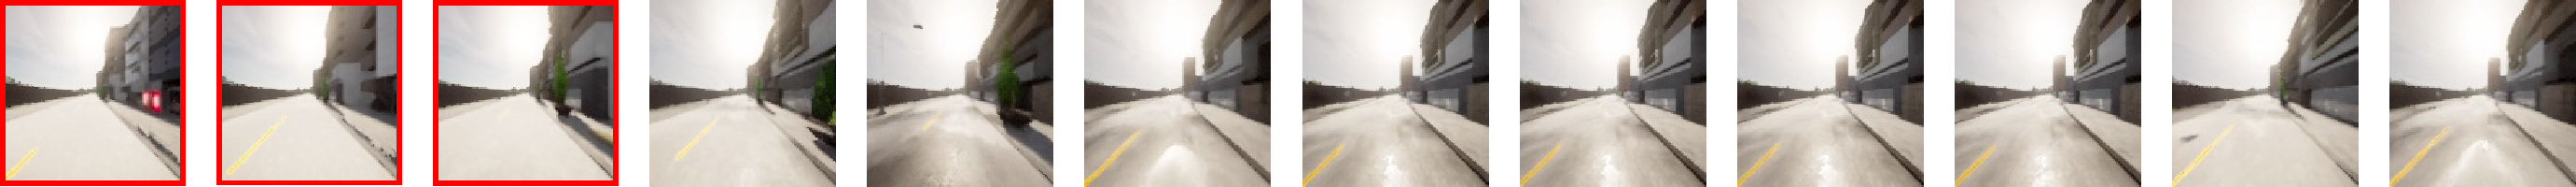
\includegraphics[width=\textwidth]{figs/thesis/fdm-example-tasks/world-modeling-thesis.pdf}
    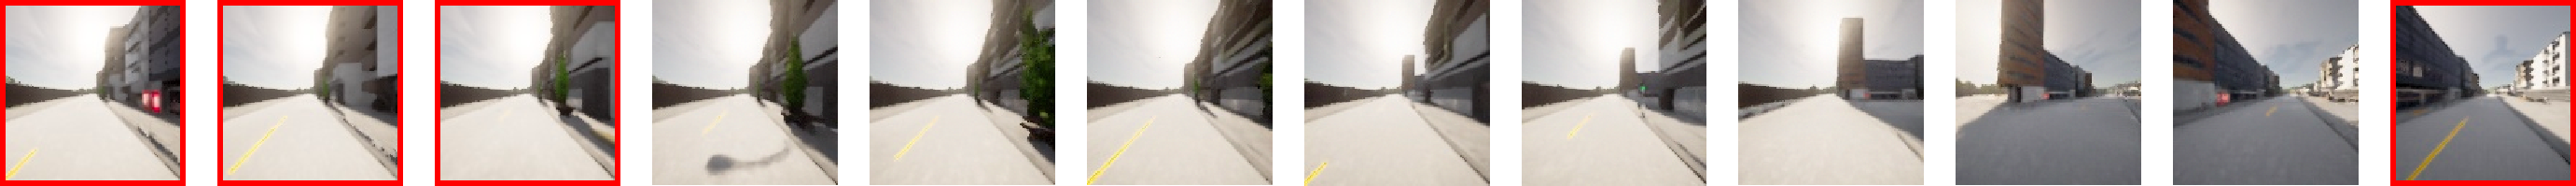
\includegraphics[width=\textwidth]{figs/thesis/fdm-example-tasks/visual-planning-thesis.pdf}
    \caption{Sampled 11-frame videos from a flexible generative model that was trained on first-person data collected by a simulated autonomous vehicle within one virtual town. \textbf{Top:} A sample conditioned on the first three frames. This can be interpreted as conditioning on the vehicle's current state and predicting what it will do and see in the future. \textbf{Bottom:} A sample conditioned on a final ``goal'' frame as well as the first three frames. Conditioning on both the current state and a goal corresponds to goal-directed planning. }
    \label{fig:intro-world-modeling-and-planning}
\end{figure}

The specific set of conditioning tasks that we may care about is domain dependent, but a reasonable goal in domains with fixed-dimensionality data is to be able to generate data $\rvx \in \mathbb{R}^d$ conditioned on specified values of any arbitrary set of components of $\rvx$, where a component may be, e.g., a pixel if $\rvx$ is an image or, e.g., a frame if $\rvx$ is a video. To be more precise,
% Denoting the data $\rvx \in \mathbb{R}^d$, a flexible generative model for this domain could ideally, at test-time,
let us use $\gY$ to refer to a list of the indices of all observed components of a particular datapoint and use $\rvy := \rvx[\gY]$ to refer to the corresponding observed values. Then we define a flexible generative model as one that can approximate $\pdata(\rvx|\rvy,\gY)$ well for any given $\gY$ and $\rvy$, without retraining.
% generate $\rvx$ conditioned on specified values of any components (e.g. image pixels) of $\rvx$. That is, denoting a list of observed components $\gY$ and their values $\rvy := \rvx[\gY]$, we should be able to sample from an approximation of $p_\data(\r)$
% $\rvx$ conditioned on $\rvy := \mM \odot \rvx$ for any binary mask $\mM \in \{0,1\}^d$, where $\odot$ represents element-wise multiplication. 
This type of flexible model could enable many new use-cases in the domains described previously. Flexible models are already widely used in image editing, in the form of image inpainting models that can be conditioned on the values of any set of image pixels and then generate plausible values for the remainder~\citep{rombach2022high,zhao2021large,harvey2021conditional}.

\Cref{fig:intro-world-modeling-and-planning} hints at the tasks that such a flexible model would be capable of in the video domain. If the video data is from the first-person perspective of an agent, having a flexible video generative model makes it possible to: condition on previous frames as a representation of the agent's current or past state; condition on near-future goals (e.g. desired locations) for planning tasks; or, using the techniques we will introduce in this thesis, even to condition on goals hundreds of frames in the future. In a reinforcement learning sense, this generative model is capable of doing all of: serving as a world model; implicitly modelling the agent's policy; and performing goal-directed planning. Future applications could include alternatives to (or integrations with) GPS-based navigation that can better incorporate visual cues in their planning, or controllers for advanced robots that take a visual input. One can similarly imagine a myriad of potential applications of flexible generative models for, e.g., digital twins or in speech-to-text-style systems, but we limit the scope of this dissertation to the vision domain.

% In the video domain, such a flexible model would be capable of tasks like generating a video conditioned on: a given image being the first frame; a given image being the last frame; the first few frames; every $n$th frame (i.e. temporal super-resolution); or any of many other imaginable tasks. These tasks take on even more significance if we consider the case where the video is the first-person view of an agent. Conditioning on the first few frames may then mean conditioning on an agent's current state and conditioning on certain values of later frames could mean conditioning on the agent fulfilling some goal like navigating to a given location. The flexible video model then has the potential to provides an alternative to traditional GPS-based navigation systems. 

We aim to demonstrate that generative models within the vision domain can be made flexible while retaining good performance, and sometimes with improved performance over our non-flexible baselines. We will focus on demonstrating this within the diffusion modelling framework, which has become dominant for models of images and video~\citep{sohl2015deep,ho2020denoising,dhariwal2021diffusion,rombach2022high,ho2022imagen,peebles2022scalable,brooks2024video}. We will therefore begin this thesis by reviewing the diffusion modelling framework in \cref{ch:diffusion}. We will show that diffusion models are naturally amenable to being used for conditional generation and even flexibly conditional generation of the type that we target in \cref{ch:conditional-diffusion,ch:flexible-diffusion}. Our central contribution will be introducing innovations that enable flexible conditioning in challenging settings. First we consider the long video domain where the complexity and dimensionality of typical datapoints is such that it is infeasible to take the standard approach of training a single model of all frames in \cref{ch:fdm}. Next we will target flexible generative modelling in domains where the dimensionality of different data points varies and so must be sampled along with the data values given any conditioning information in \cref{ch:tddm}; this is challenging for traditional conditional generative models. Finally, we recognise that the diffusion modelling may not remain the dominant paradigm for generative modelling of images and video forever. We therefore end by demonstrating that a different generative model class, variational auto-encoders, are also amenable to being used to build flexible generative models in \cref{ch:cigcvae}.

% \section*{Thesis outline}
% In \cref{ch:diffusion} we describe diffusion models as unconditional generative models which can be fit to a data distribution $\pdata(\rvx)$. In \cref{ch:conditional-diffusion} we will build on this by reviewing conditional diffusion models which parameterise an approximation of the conditional distribution $\pdata(\rvx|\rvy)$ given conditioning information $\rvy$. In \cref{ch:flexible-diffusion} we will define and explain the flexible diffusion framework, including our proposed training objective for flexible diffusion models and examples of flexible diffusion models. We propose two modifications in later chapters: in \cref{ch:fdm} we review the problem of learning generative models for long videos and then propose modifications to our flexible diffusion framework to adapt it to this domain. In \cref{ch:tddm} we study the task of conditionally generating varying-dimensional data, where we need the conditional generative model to be capable of sampling an appropriate number of dimensions that in general will depend on the information that is conditioned on. In \cref{ch:cigcvae} we review the VAE framework as an alternative to diffusion models, allowing us to present evidence that flexible generative modelling is practical with frameworks other than just diffusion modelling. We then present our final conclusions in \cref{ch:conclusion}.